
%(BEGIN_QUESTION)
% Copyright 2010, Tony R. Kuphaldt, released under the Creative Commons Attribution License (v 1.0)
% This means you may do almost anything with this work of mine, so long as you give me proper credit

Determine the value of the specified {\it integral} for this function:

$$\includegraphics[width=15.5cm]{i04374x01.eps}$$

$$\int_{+2}^{-2} f(x) \> dx$$

\underbar{file i04374}
%(END_QUESTION)





%(BEGIN_ANSWER)

$-3$

\vskip 10pt

Note how the interval of integration starts at $x = +2$ and proceeds to $x = -2$.  This means the integration proceeds in a negative direction, from +2 to -2 on the horizontal axis.  Another way of saying this is that each differential of $x$ is a negative quantity ($dx < 0$).  This explains why the integral value is a negative quantity (-3) despite the fact that $y$ never goes below zero during the entire interval of integration.

%(END_ANSWER)





%(BEGIN_NOTES)


%INDEX% Mathematics, calculus: integral (approximating integral values between points on graph)

%(END_NOTES)


